\documentclass{beamer}

\usepackage{amsmath, amssymb}
\usepackage{graphicx}
\usepackage{url}
\usepackage{xspace}
\usepackage{pifont}
\usepackage{minted}
\usepackage{verbatim}
\usepackage{wasysym}
\usepackage[notocbib]{apacite}
\usepackage{movie15}
\usepackage{animate}
\usepackage{bm}

\DeclareMathOperator{\Tr}{Tr}
\DeclareMathOperator*{\argmin}{arg\,min}

\usetheme{AnnArbor}
\usefonttheme[onlymath]{serif}

\title[Intro DNNs]{\textbf{Practical Deep Neural Networks} \\
\textbf{\normalsize GPU computing perspective}\\
\normalsize Softmax Regression}
\author{Yuhuang Hu \and Chu Kiong Loo}
\institute[UM]{Advanced Robotic Lab\\
Department of Artificial Intelligence\\
Faculty of Computer Science \& IT\\
University of Malaya}

\date{}

\begin{document}

\frame{\titlepage}

\begin{frame}
  \frametitle{Outline}

  \tableofcontents
\end{frame}

\AtBeginSection[]
  {
     \begin{frame}
     \frametitle{Outline}
     \tableofcontents[currentsection]
     \end{frame}
  }

\section{Introduction}

\begin{frame}
  \frametitle{Assumed Prerequisites}

  \begin{itemize}
    \item[\ding{80}] Basic Linear Algebra (DL book chapter 2)
    \item[\ding{80}] Basic Probability and Information Theory (DL book chapter 3)
    \item[\ding{80}] Basic Numerical Computation (DL book chapter 4)
    \item[\ding{80}] Machine Learning Basics (DL book chapter 5)
  \end{itemize}
\end{frame}

\begin{frame}
  \frametitle{Suggested Readings}

  \begin{itemize}
    \item[\ding{45}] UFLDL Tutorial: \href{http://ufldl.stanford.edu/tutorial/supervised/LogisticRegression/}{Logistic Regression}, \href{http://ufldl.stanford.edu/tutorial/supervised/SoftmaxRegression/}{Softmax Regression} and \href{http://ufldl.stanford.edu/tutorial/supervised/OptimizationStochasticGradientDescent/}{Stochastic Gradient Descent}.
    \item[\ding{45}] CS231n: \href{http://cs231n.github.io/linear-classify/}{Linear classification: Support Vector Machine, Softmax} and \href{http://cs231n.github.io/optimization-1/}{Optimization: Stochastic Gradient Descent}.
    \item[\ding{45}] \href{http://www.iro.umontreal.ca/~bengioy/dlbook/numerical.html}{DL Book Chapter 4 Numerical Computation 4.3} \href{http://www.iro.umontreal.ca/~bengioy/dlbook/optimization.html}{DL Book Chapter 8 Numerical Optimization 8.3}
  \end{itemize}
\end{frame}

\section{Logistic Regression}

\begin{frame}
  \frametitle{Logistic Function}

  \begin{align*}
    f(\mathbf{x})&=\frac{1}{1+\exp(-\mathbf{W}^{\top}\mathbf{x})} \\
    p(y=1|\mathbf{x})&=f(\mathbf{x})\\
    p(y=0|\mathbf{x})&=1-f(\mathbf{x})
  \end{align*}
\end{frame}

\begin{frame}
  \frametitle{Logistic Regression --- Binary Classifier}

  \begin{align*}
    L(X, \mathbf{y}|\mathbf{W})&=-\frac{1}{N}\sum_{i}\left(y^{i}\log(P(y=1|\mathbf{x}^{i}))+(1-y^{i})\log(p(y=0|\mathbf{x}^{i}))\right) \\
    W^{\star}&=\argmin_{W}L(X, \mathbf{y})
  \end{align*}
\end{frame}

\section{Softmax Regression}

\begin{frame}
  \frametitle{Extending Logistic Function --- Softmax Function}

  \begin{equation*}
    P(y=k|\mathbf{x}; \mathbf{W})=\frac{\exp(\mathbf{W}^{(k)\top}\mathbf{x})}{\sum_{j=1}^{K}\exp(\mathbf{W}^{(j)\top}\mathbf{x})}
  \end{equation*}
\end{frame}

\begin{frame}
  \frametitle{Softmax Regression --- Multi-classes Classifier}

  \begin{align*}
    L(X, \mathbf{y}|\mathbf{W})&=-\frac{1}{N}\sum_{i}\sum_{k=1}^{K}\mathbf{1}\{y^{i}=k\}\log P(y^{i}=k|\mathbf{x}^{i}, \mathbf{W}) \\
    \mathbf{W}^{\star}&=\argmin_{\mathbf{W}}L(X, \mathbf{y})
  \end{align*}
\end{frame}

\section{Stochastic Gradient Descent}

\begin{frame}
  \frametitle{Cost}
  \begin{itemize}
    \item Target: to learn some optimal parameters $\theta$
    \item Strategy: to minimize some cost $L$ respect to $\theta$
    \item Cost choice: cross-entropy cost, mean-squared error cost
    \item Solution: Gradient Descent!
  \end{itemize}
\end{frame}

\begin{frame}
  \frametitle{Gradient optimization}
  \begin{figure}
    \centering
    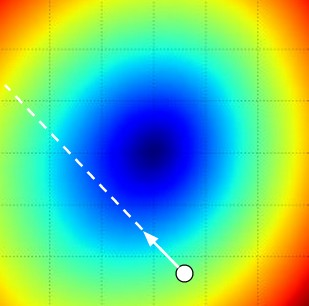
\includegraphics[width=0.5\textwidth]{stepsize.jpg}
  \end{figure}

  \href{http://rt.dgyblog.com/res/dlworkshop/opt1.gif}{Demo 1}; \href{http://rt.dgyblog.com/res/dlworkshop/opt2.gif}{Demo 2}
\end{frame}

\begin{frame}
  \frametitle{Stochastic Gradient Descent (SGD)}

  \begin{equation*}
    \theta^{*}=\theta-\alpha\frac{\partial}{\partial \theta}L(\theta)
  \end{equation*}
\end{frame}


\begin{frame}
  \frametitle{Variants: momentum SGD}

  \begin{align*}
    V^{*}&=\mu V-\alpha\nabla L(\theta) \\
    \theta^{*}&=\theta+V^{*}
  \end{align*}
\end{frame}

\begin{frame}
  \frametitle{Variants: Nesterov's Accelerated Gradient (NAG)}
  \begin{align*}
    V^{*}&=\mu V-\alpha\nabla L(\theta+\mu V) \\
    \theta^{*}&=\theta+V^{*}
  \end{align*}
\end{frame}

\section*{Q\&A}

\begin{frame}
  \frametitle{Q\&A}
  \begin{figure}
    \centering
    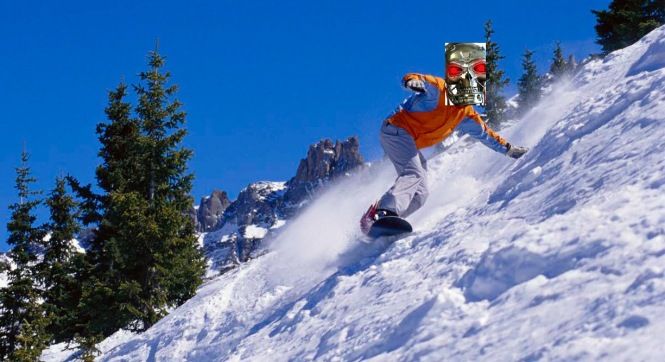
\includegraphics[width=0.7\textwidth]{gradient_descent.jpg}
  \end{figure}
\end{frame}


\end{document}

%%% Local Variables:
%%% mode: latex
%%% TeX-master: t
%%% End:
